\newpage
\chapter{Статистическа обработка на данните}
\label{chapter09}

Статистическата обработка на данни се състои основно от два вида статистика – описателна статистика и сравнителна статистика. При описателната статистика се изчисляват определени параметри описващи характеристики на събраните данни, докато при сравнителната статистика се извършва сравнение между някои от описателните параметри на данните. 

\section{Описателна статистика}

Параметрите при описателната статистика основно са свързани с някакво централно групиране на данните и някакво разпръскване (дисперсия) около централното групиране. Параметри за централно групиране са средната стойност, медианата и модата, а параметри за разпръскване са дисперсията и стандартното отклонение.

\begin{lstlisting}[caption=Генериране на извадка от случайни числа, label=listing0160]
v1 <- round( rnorm(100, mean=62, sd=72) )

v2 <- v1

v2[sample(x=1:100, size=15, replace=FALSE)] <- NA

w1 <- 1 / sample(x=1:100, size=100, replace=TRUE)
\end{lstlisting}

За да бъдат илюстрирани възможностите на R за пресмятане на описателни статистики се използва извадка от 100 нормално разпределени случайни числа (Листинг \ref{listing0160}). Често в реалната практика данните съдържат липсващи измервания. При такава ситуация трябва да се вземат допълнителни мерки за пресмятане на описателните статистики. Функцията sample в R позволява на случаен принцип част от стойностите в определен вектор да бъдат избрани на случаен принцип, при равномерно вероятностно разпределение. Тази възможност се използва за замяна на 15\% от генерираните данни с липсваща стойност (Листинг \ref{listing0160}). Параметърът replace указва дали определено число може да бъде избрано повторно или не.

\subsection{Средна стойност}

Средната стойност е най-често използваната статистика и представлява сумата от стойностите разделена на общия брой стойности (Листинг. \ref{listing0161}).

\begin{lstlisting}[caption=Средна стойност, label=listing0161]
sum(v1) / length(v1)

mean( v1 )

mean( v2 )

mean(v2, na.rm=TRUE)
\end{lstlisting}

Когато липсват стойности при проведените измервания е невъзможно да се изчисли средната стойност без да се вземе решение как да се обработят липсващите числа. Има различни подходи за обработката на липсите, като интерполация или премахване. Независимо кой подход бъде избран, то той неизбежно води до внасяне на допълнителна грешка при пресмятанията. Ако бъде извършена интерполация, то съседните измервания биха внесли грешка в липсващите стойности. Ако бъдат премахнати липсващите измервания, то размерът на извадката намалява, а от там се увеличава и неточността на последващите пресмятания. 

В някои ситуации отделните измерени стойности имат различна тежест и се налага те да участват с различен коефициент при пресмятането на средната стойност (Листинг \ref{listing0162}). Такава е ситуацията когато се пресмята бал за прием в учебно заведение. Различните компоненти формиращи бал на всеки кандидат участват с различна тежест.

\begin{lstlisting}[caption=Претеглена средна стойност, label=listing0162]
weighted.mean(x=v1, w=w1)
\end{lstlisting}

\subsection{Минимална стойност, максимална стойност, медиана и мода}

В практиката често от значение е диапазонът в който се разпростират данните. В програмния пакет R този диапазон лесно се установява с функциите min и max (Листинг \ref{listing0163}).

\begin{lstlisting}[caption={Минимум, максимум, медиана и мода}, label=listing0163]
min( v1 )

max( v1 )

median( v1 )

# Mode calculation.
unique(v1)[ which.max( tabulate(match(v1,unique(v1)) ) ) ]
\end{lstlisting}

Един от основните недостатъци на средната стойност е, че при наличието на екстремално различни отделни измервания силно могат да повлияят върху общото пресмятане на средната стойност. Поради тази причина в практиката много често се използва медианата, а не средната стойност (Листинг \ref{listing0163}). За да се пресметне медианата данните се сортират. При нечетен брой стойности медианата е стойността на средния елемент. При четен брой стойности медианата е средно аритметично между двата елемента в средата. 

Модата е параметър, който отразява най-често срещаната стойност в множеството от данни. Освен числена стойност модата може да има и символна стойност, според характера на самите данни. В програмния пакет R няма функция, която да изчислява модата, но тя лесно може да се пресметне с комбинация от извикването на други функции (Листинг \ref{listing0163}).

\subsection{Дисперсия и стандартно отклонение}

След като бъде установено някакво централно групиране в данните е от съществено значение по какъв начин данните са разпръснати около това централно групиране. Изчисляването на дисперсията спомага за изследване на разпръскването (Листинг \ref{listing0164}). Дисперсията се изчислява като сума от квадрата на разликите между всяка стойност и средната, разделена на броя стойности минус едно. 

\begin{lstlisting}[caption=Дисперсия и стандартно отклонение, label=listing0164]
sum( (v1-mean(v1))^2 ) / (length(v1) - 1)

var( v1 )

sqrt( var(v1) )

sd( v1 )
\end{lstlisting}

Основен недостатък на дисперсията е, че се изчислява с повдигане на втора степен и полученият резултат е несравним с оригиналните измервания. Примерно при серия измервания в метри резултатът от изчислението на дисперсията би имал смисъла на квадратни метри. За да бъдат сравними стойностите е достатъчно дисперсията да се подложи на корен квадратен, което коригира резултата получен с повдигане на втора степен. Резултатът от квадратния корен на дисперсията се нарича стандартно отклонение (Листинг \ref{listing0164}).

\subsection{Квантили и обобщение}

Квантилите определят каква част от измерените стойности попадат в определен процент от вероятностното разпределение (Листинг \ref{listing0164}).

\begin{lstlisting}[caption=Квантили и обобщение, label=listing0165]
quantile(v1, probs=c(0.1, 0.2, 0.3, 0.4, 0.5, 0.6, 0.7, 0.8, 0.9))
#  10%   20%   30%   40%   50%   60%   70%   80%   90% 
#-28.0  -0.4  19.0  41.6  66.5  84.4 110.6 121.8 150.2 

summary( v1 )
\end{lstlisting}

Програмният пакет R предоставя и обобщаваща функция за описателните статистики наречена summary и тя визуализира стойностите за минимална, максимална, медиана, средна, първи и трети квантил.

\section{Сравнителна статистика}

Когато се работи с две или повече случайни променливи от ползва идва апарата на сравнителната статистика. Целта е да се изследва връзката между тези променливи. За променливи от едно и също измерване най-често се използват корелацията и ковариацията, а за сравнение на средни T-тест и ANOVA. 

\subsection{Ковариация и корелация}

Корелационният коефициент е число в интервала -1 до +1 и показва възможността за наличие на взаимна връзка между две случайни променливи. Важно е да се отбележи, че корелационният коефициент не гарантира наличие на взаимна връзка, а само указва, че такава връзка е възможна. 

\begin{lstlisting}[caption=Ковариация и корелация, label=listing0166]
library(ggplot2)

cor(economics$psavert, economics$pce)

# Correlation formula.
sum((economics$psavert-mean(economics$psavert)) * (economics$pce-mean(economics$pce))) / ((nrow(economics)-1) * sd(economics$psavert) * sd(economics$pce))

cor(economics[, c("pce","psavert","uempmed","unemploy")])

cov(economics$psavert, economics$pce)

cov(economics[, c("pce","psavert","uempmed","unemploy")])

# Correlation is a covariance divided by the standard deviation.
identical(cov(economics$psavert,economics$pce),cor(economics$psavert,economics$pce)*sd(economics$psavert)*sd(economics$pce))
\end{lstlisting}

В пакета ggplot2 множеството от данни economics дава идеална възможност да се демонстрира концепцията за корелация и ковариация (Листинг \ref{listing0166}). Колоната psavert отразява индивидуалното спестовно ниво, а колоната pce индивидуалните разходи. При относително еднакво ниво на доходите, чисто интуитивно е ясно, че който харчи повече би следвало да спестява по-малко. Това ще рече, че когато едната стойност нараства другата стойност ще намалява и това има смисъла на отрицателна корелационна връзка. В демонстрирания пример корелационният коефициент е -0.7928546 и отразява точно факта за възможно наличие на относително силна отрицателна корелационна връзка. 

\begin{equation}
r_{xy} = \frac{\sum_{i=1}^{n}(x_i-\bar{x})(y_i-\bar{y})}{(n-1)s_xs_y}
\label{equation0009}
\end{equation}
\listofequations{Корелационен коефициент}

Корелационният коефициент се пресмята като сума от разликите между множителите на отделните измервания в разлика от средната стойност, разделена на умножението между стандартните отклонения на двете променливи с броя измервания минус единица (Формула \ref{equation0009}). При стойност близка до +1 е възможна силна положителна корелационна връзка, при стойност близка до -1 е възможна силна отрицателна корелационна връзка, а при стойност близка до 0 наличието на корелационна връзка е много малко вероятно. 

Когато корелацията се смята между повече от две случайни променливи резултатът е корелационна матрица (Листинг \ref{listing0166}). При корелационната матрица е показана възможната връзка между всяка двойка променливи. 

\begin{equation}
v_{xy} = \frac{1}{n-1}\sum_{i=1}^{n}(x_i-\bar{x})(y_i-\bar{y})
\label{equation0010}
\end{equation}
\listofequations{Ковариационен коефициент}

Ковариацията е подобна на корелацията, като разликата е, че стойностите не са нормирани (Формула \ref{equation0010}). Може да се приеме като аналогия между дисперсията и стандартното отклонение (Листинг \ref{listing0166}). Ковариацията може да бъде голямо отрицателно число или голяма положително число. В посочения пример ковариацията е със стойност -8359.069, при съответната ковариационна матрица. 

Както при описателните статистики, при ковариацията и корелацията липси в измерванията възпрепятстват изчисляването на крайните стойности. 

\subsection{Тест на Стюдънт}

От сравнителната статистика t-теста (или тест на Стюдънт) е един от най-разпространените подходи за сравнение на средните стойности между две извадки. 

\begin{lstlisting}[caption=Тестово множество за бакшиши, label=listing0167]
library(reshape2)

head(tips)
\end{lstlisting}

За илюстриране на възможностите, които R предлага при пресмятането на t-теста е подходящо да се използва множеството данни за бакшиши (Листинг \ref{listing0167}).

\subsubsection{Тест на една извадка}

При тестването на една извадка теста се прилага за определяне на средната стойности и съответният доверителен интервал. От съществено значение е данните да са нормално разпределение което означава, че имат конкретна средна стойност и конкретно стандартно отклонение. Ако тестваната стойност попада в доверителния интервал, то може да се заключи, че това е действителната средна стойност. В противен случай не може да се приеме, че предположената средна стойност е действителната средна стойност. 

\begin{lstlisting}[caption=Тест на единична извадка, label=listing0168]
t.test(tips$tip, alternative="two.sided", mu=3.50)

# 	One Sample t-test
# 
# data:  tips$tip
# t = -5.6642, df = 243, p-value = 4.161e-08
# alternative hypothesis: true mean is not equal to 3.5
# 95 percent confidence interval:
#  2.823799 3.172758
# sample estimates:
# mean of x 
#  2.998279 
\end{lstlisting}

При проверката дали средната стойност на бакшишите е \$3.5 $t$-тестът завършва с отчет за пресметнатите стойности (Листинг \ref{listing0168}), което включва - $t$ статистиката, степените на свобода и $p$ стойността. Също така е представена информация за 95 процентният доверителен интервал и информация за средната стойност на изследваната променлива. Постигнатата p стойност означава, че нулевата хипотеза трябва да бъде отхвърлена. Това води до заключението, че средната стойност на бакшишите не може да е \$3.5. Нулевата хипотеза е това, което се смята за истина (в примера това е средна стойност е равна на \$3.5). 

\begin{equation}
t = \frac{\bar{x}-\mu_0}{s_{\bar{x}}/\sqrt{n}}
\label{equation0011}
\end{equation}
\listofequations{T-статистика}

T-статистиката се смята по формула \ref{equation0011} и има смисъла на отношение между разликата от пресметнатото средно ($\bar{x}$) и предположеното средно ($\mu_0$), а като делител е стандартната грешка на пресметнатото средно ($s_{\bar{x}}/\sqrt{n}$). В уравнението $s_{\bar{x}}$ има смисъла на стандартно отклонение, а $n$ е броят на наблюденията. 

\begin{figure}[h!]
  \centering
  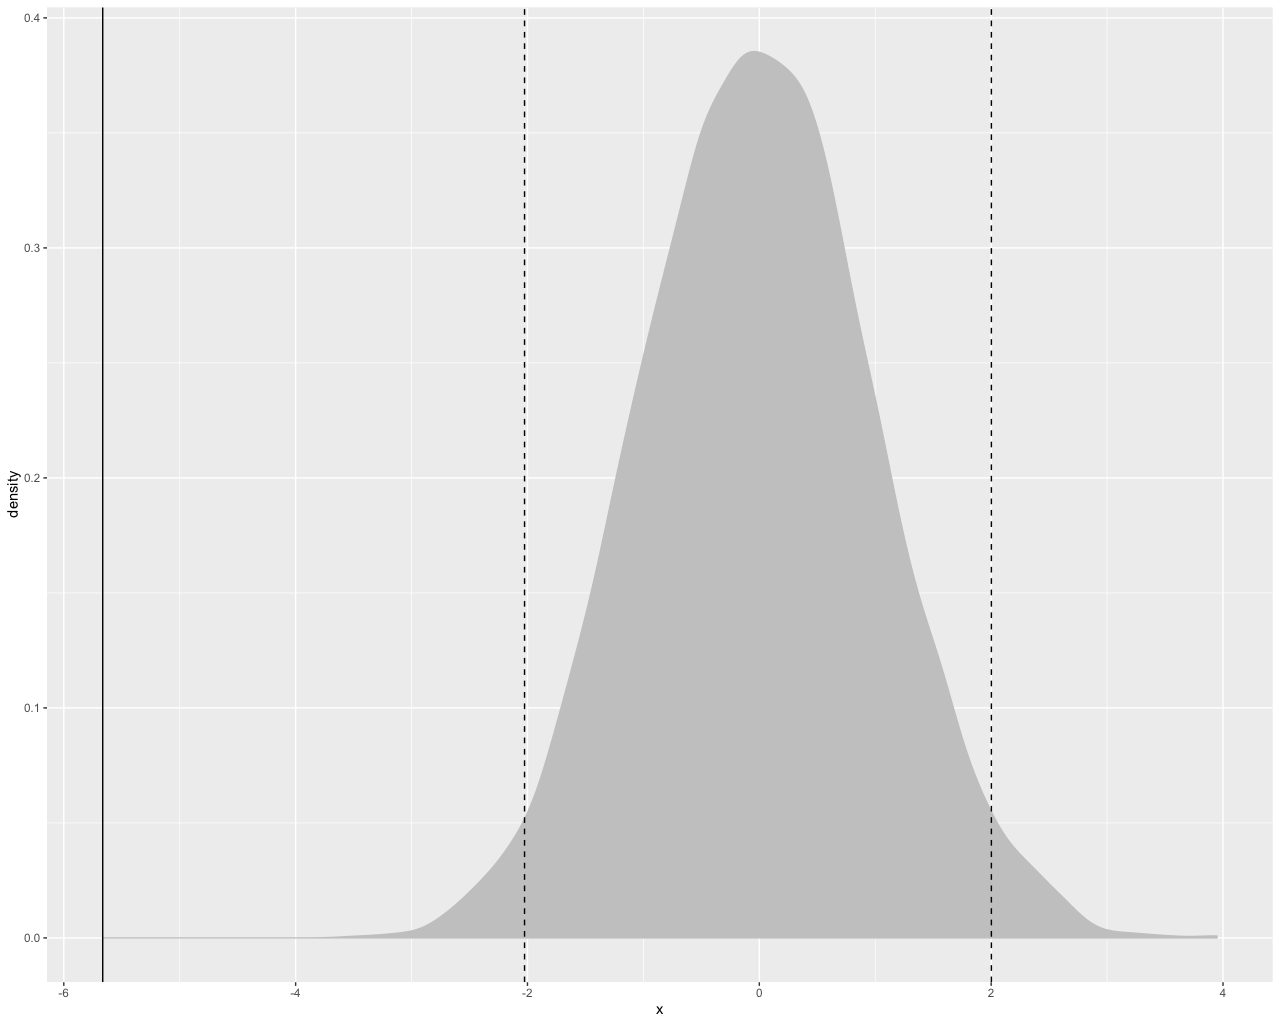
\includegraphics[width=1.0\linewidth]{pic0056}
  \caption{Т-статистика за бакшиши}
\label{figure0056}
\end{figure}
\FloatBarrier

Когато предположената средна стойност е вярна очакването е $t$-статистиката да попада в интервала от две стандартни отклонения, около средната стойност (Фиг. \ref{figure0056}). 

\begin{lstlisting}[caption=Визуализация на t-разпределение, label=listing0169]
library( ggplot2 )

# Generation of t-distributed random values.
values <- rt(10000, df = NROW( tips ) - 1)

# T-statistics calculation.
t <- t.test(tips$tip, alternative="two.sided", mu=3.50)

# Visualization.
ggplot(data.frame(x=values)) + geom_density(aes(x=x), fill="grey", color="grey") + geom_vline(xintercept=t$statistic) + geom_vline(xintercept=mean(values) + c(-2, 2) * sd(values), linetype=2)
\end{lstlisting}



